\subfigure[]{
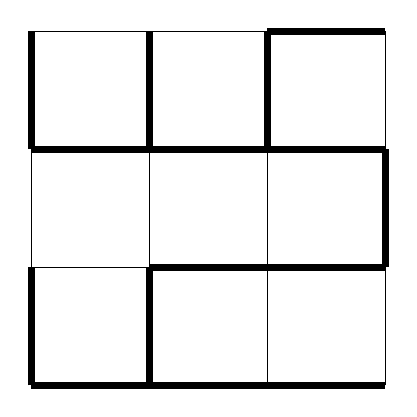
\begin{tikzpicture}
[linedecorate/.style={line width=2.5pt}]
%% set up the grid
\foreach \xstart/\xend/\y in {0/4.5/0, 0/4.5/1.5, 0/4.5/3, 0/4.5/4.5} {
  \draw (\xstart,\y) -- (\xend,\y);
  \draw (\y,\xstart) -- (\y,\xend);
}
%% draw the spanning tree
\foreach \xstart/\ystart/\xend/\yend in {0/0/0/1.5, 0/0/4.5/0,
  1.5/0/1.5/1.5, 1.5/1.5/4.5/1.5, 4.5/1.5/4.5/3, 0/3/4.5/3, 0/3/0/4.5,
  1.5/3/1.5/4.5, 3/3/3/4.5, 3/4.5/4.5/4.5}
{
  \draw[linedecorate] (\xstart,\ystart) -- (\xend,\yend);
}
\end{tikzpicture}
}
%%
%%
\qquad
\subfigure[]{
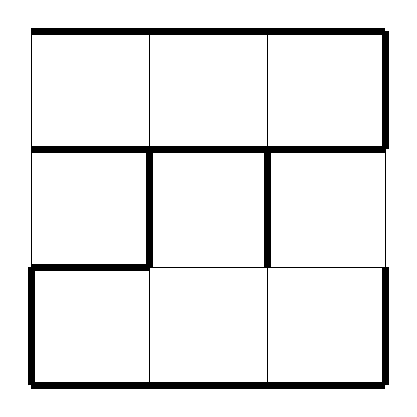
\begin{tikzpicture}
[linedecorate/.style={line width=2.5pt}]
\foreach \xstart/\xend/\y in {0/4.5/0, 0/4.5/1.5, 0/4.5/3, 0/4.5/4.5} {
  \draw (\xstart,\y) -- (\xend,\y);
  \draw (\y,\xstart) -- (\y,\xend);
}
%% draw the spanning tree
\foreach \xstart/\ystart/\xend/\yend in {0/0/0/1.5, 0/0/4.5/0,
  4.5/0/4.5/1.5, 0/1.5/1.5/1.5, 1.5/1.5/1.5/3, 3/1.5/3/3, 0/3/4.5/3,
  4.5/3/4.5/4.5, 0/4.5/4.5/4.5}
{
  \draw[linedecorate] (\xstart,\ystart) -- (\xend,\yend);
}
\end{tikzpicture}
}
